\documentclass{beamer}
\mode<presentation>{
    \usetheme{Madrid}
    \setbeamertemplate{footline}{}
    \setbeamertemplate{navigation symbols}{}}

\usepackage[utf8]{inputenc}
% Allows including images.
\usepackage{graphicx}
\setcounter{tocdepth}{2}
%% Display notes.
%\usepackage{pgfpages}
%\setbeameroption{show notes on second screen}
% Stop messing with my single quotes!
\usepackage{upquote}

\newcommand{\autotitle}
{\frametitle{
    \secname
    \ifx\insertsubsection\empty
    \else
        /\subsecname
        \ifx\insertsubsubsection\empty\else/\subsubsecname\fi
    \fi}}

\title{Linux containers}
\subtitle{You are not expected to understand this}

\author{Bruno Barcarol Guimarães}
\institute[]{\textit{bbguimaraes.com}}
\date{2016-10-06}

\begin{document}

\begin{frame}
    \titlepage
\end{frame}

\section{overview}

\begin{frame}
    \autotitle
    \tableofcontents
\end{frame}

\subsection{introduction}

\begin{frame}
    \autotitle
    You are not expected to understand this.
\end{frame}

\begin{frame}
    \autotitle
    \begin{quote}
        You are not expected to understand this.
    \end{quote}
    Dennis Ritchie
    \note{
        Dennis Ritchie was a colleague of Ken Thompson (creator of UNIX), at
        Bell Labs, AT\&T.
        \\~\\
        He was one of the earliest contributors to UNIX and creator of the C
        programming language.}
\end{frame}

\begin{frame}[fragile]
    \autotitle
    \begin{quote}
        \tiny
        \begin{verbatim}
/*
 * Switch to stack of the new process and set up
 * his segmentation registers.
 */
retu(rp->p_addr);
sureg();
/*
 * If the new process paused because it was
 * swapped out, set the stack level to the last call
 * to savu(u_ssav).  This means that the return
 * which is executed immediately after the call to aretu
 * actually returns from the last routine which did
 * the savu.
 *
 * You are not expected to understand this.
 */
if(rp->p_flag&SSWAP) {
    rp->p_flag =& ~SSWAP;
    aretu(u.u_ssav);
}
/*
 * The value returned here has many subtle implications.
 * See the newproc comments.
 */
return(1);
        \end{verbatim}
    \end{quote}
    Dennis Ritchie, Sixth Edition Unix (1975)
    \cite{dennis_you_are_not_expected}
\end{frame}

\begin{frame}
    \autotitle
    \begin{quote}
        "You are not expected to understand this" was intended as a remark in
        the spirit of "This won't be on the exam," rather than as an impudent
        challenge.
    \end{quote}
    Dennis Ritchie
    \cite{dennis_you_are_not_expected_explanation}
\end{frame}

\begin{frame}
    \autotitle
    \begin{quote}
        The real problem is that we didn't understand what was going on either.
        \\~\\
        \scriptsize
        The savu/retu mechanism for doing process exchange was fundamentally
        broken because it depended on switching to a previous stack frame and
        executing function return code in a different procedure from the one
        that saved the earlier state.  This worked on the PDP-11 because its
        compiler always used the same context-save mechanism; with the
        Interdata compiler, the procedure return code differed depending on
        which registers were saved.
        \\~\\
        So, for Steve Johnson and me, trying to move the kernel for the first
        time to a new machine, this code was indeed on the exam.  It took about
        a week of agonizing before we finally convinced each other that the
        mechanism was wrong and no fiddling with the compiler was useful.  We
        redid the coroutine control-passing primitives altogether, and this
        code section, and the comment, passed into history.
    \end{quote}
    Dennis Ritchie
\end{frame}

\subsection{pre-history}

\begin{frame}
    \autotitle
    \begin{quote}
        You have probably heard about Docker and Containers, but FreeBSD
        have had jails since I wrote them in 1998.
    \end{quote}
    Poul-Henning Kamp
    \cite{kamp_varnish}
\end{frame}

\subsubsection{time-sharing}

\begin{frame}
    \autotitle
    \begin{itemize}
        \item
            First appearance of the term by Josh Backus in a MIT Summer Session
            (1954)
        \item
            Project to implement a time-sharing system started by John McCarthy
            at MIT (1959)
        \item Compatible Time-Sharing System, CTSS (1961)
    \end{itemize}
    \note{
        The concepts behind containers date back to the first time-sharing
        systems in the early days of modern computer history.}
\end{frame}

\begin{frame}
    \autotitle
    \begin{picture}(330, 200)
        \put(0, 0){
            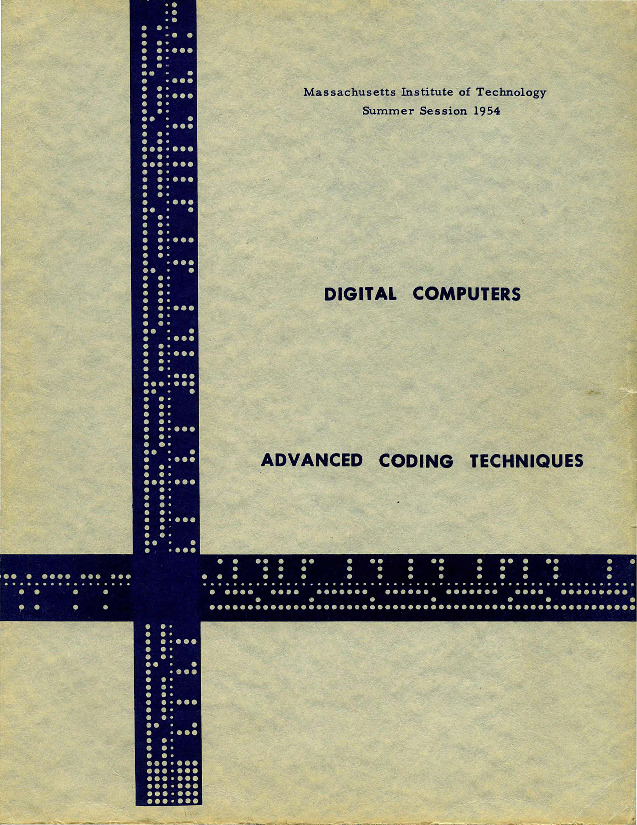
\includegraphics[width=.45\linewidth]
                {img/advanced_coding_techniques0.jpg}}
        \only<2>{
            \put(25, 5){
                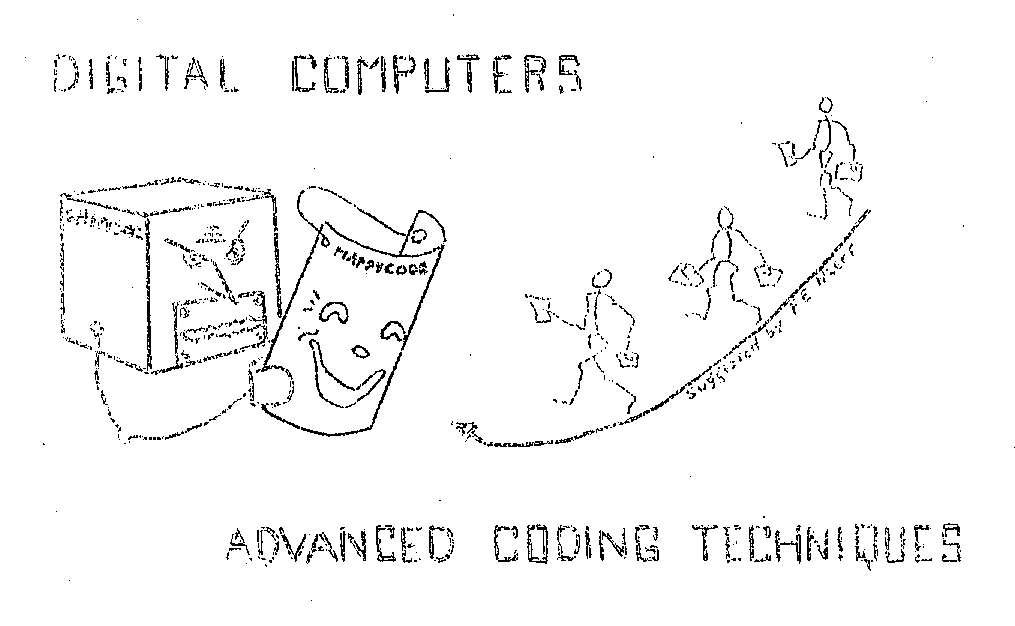
\includegraphics
                    [width=.90\linewidth]
                    {img/advanced_coding_techniques1.png}}}
    \end{picture}
\end{frame}

\begin{frame}
    \autotitle
    \begin{quote}
        Mr. P. F. Williams said that his firm is trying to decide on a
        computer to use.  They want something intermediate between an
        IBM 650 and 704.  The 704 seems too large: they would not be
        able to keep it busy.  Josh Backus said that by time sharing, a
        big computer could be used as several small ones; [...]
    \end{quote}
    Computer Advanced Coding Techniques, MIT Summer Session
    \cite{mit_summer_session}
    \note{
        This was in 1954, fifteen years before UNIX.  The basic concept,
        however, is still relevant.}
\end{frame}

\begin{frame}
    \autotitle
    \begin{quote}
        By allowing a large number of users to interact concurrently with a
        single computer, time-sharing dramatically lowered the cost of
        providing computing capability.  [...] While any single user would make
        inefficient use of a computer, a large group of users together would
        not.
    \end{quote}
    Wikipedia \cite{wikipedia_time_sharing}
\end{frame}

\subsection{history}

\subsubsection{chroot}

\begin{frame}
    \autotitle
    \begin{itemize}
        \item \texttt{chroot(2)}
        \item Changes the root directory of the calling process
        \item Compartmentalize the filesystem
        \item Didn't provide any other isolation mechanisms
        \item Very trivial to "escape"
        \item The goal was not security
        \item Actually, no one really knows what the goal was
    \end{itemize}
\end{frame}

\begin{frame}
    \autotitle
    \begin{quote}
        [CHROOT]
        \\~\\
        Dr. Marshall Kirk Mckusick, private communication: "According to the
        SCCS logs, the chroot call was added by Bill Joy on March 18, 1982
        approximately 1.5 years before 4.2BSD was released.  That was well
        before we had ftp servers of any sort (ftp did not show up in the
        source tree until January 1983).  My best guess as to its purpose was
        to allow Bill to chroot into the /4.2BSD build directory and build a
        system using only the files, include files, etc contained in that tree.
        That was the only use of chroot that I remember from the early days."
    \end{quote}
    Poul-Henning Kamp, Robert Watson \cite{kamp_jails}
    \note{
        In 1975, Dennis Ritchie was a visiting professor at Berkeley, where he
        met Bill Joy, then a student.
        \\~\\
        From the work that was done at this period would result the Berkeley
        Software Distribution (BSD).
        \\~\\
        Bill Joy is the author of vi and csh, and in 1982 also co-founded of
        Sun Microsystems.}
\end{frame}

\subsubsection{jails}

\begin{frame}
    \autotitle
    \begin{itemize}
        \item \texttt{jail(2)}
        \item Added to FreeBSD by Poul-Henning Kamp (1999)
        \item "Confining the omnipotent root"
        \item
            Created to address the problem of needing many machines, each
            almost idle, to have different versions of apache, mysql, perl etc.
        \item
            "Trivial extension" to \texttt{chroot(2)} to become "light-weight
            virtual 'machines'"
    \end{itemize}
\end{frame}

\begin{frame}
    \autotitle
    \begin{quote}
        The FreeBSD "Jail" facility provides the ability to partition the
        operating system environment, while maintaining the simplicity of the
        UNIX "root" model.  In Jail, users with privilege find that the scope
        of their requests is limited to the jail, allowing system
        administrators to delegate management capabilities for each virtual
        machine environment.
    \end{quote}
    Poul-Henning Kamp, Robert Watson \cite{kamp_jails}
\end{frame}

\begin{frame}
    \autotitle
    \begin{itemize}
        \item "one-way mirror effect"
        \begin{itemize}
            \item
                unjailed processes can see jailed processes, send signals,
                attach debuggers, etc. (still subject to Unix access controls)
            \item
                jailed processes can't see or interact with processes outside,
                either unjailed or in other jails
        \end{itemize}
    \end{itemize}
\end{frame}

\begin{frame}
    \autotitle
    \begin{quote}
        If somebody breaks into your computer, you face a nasty set of
        problems. For instance if you open a terminal connection, you may be
        talking to their special version of the sshd(8) daemon, and who knows
        what that does?
        \\~\\
        If you are running on perfectly virtualized servers, such as VMware,
        Xen or similar, you are as much subject to these problems as you are
        with dedicated hardware.
        \\~\\
        But if you put your outward facing services in a jail, you can
        comfortably log in using the unadultered sshd(8) in the unjailed part
        of the system, and see what the attackers are up to, while they cannot
        see you.
    \end{quote}
    Poul-Henning Kamp \cite{kamp_sagas_jails}
\end{frame}

\subsubsection{linux}

\begin{frame}
    \autotitle
    \begin{itemize}
        \item Virtuozzo
        \begin{itemize}
            \item SWsoft, now Parallels (2000)
            \item originally proprietary
            \item
                switched to open-core (OpenVZ, GPL) model (2005) \cite{openvz}
        \end{itemize}
        \item Virtual private servers and security contexts
        \begin{itemize}
            \item Jacques Gélinas (2001) \cite{virtual_private_servers}
        \end{itemize}
        \item Linux-VServer
        \begin{itemize}
            \item Herbert Pötzl (2002) \cite{linux_vserver}
        \end{itemize}
        \item all require (to this day) a patched kernel
    \end{itemize}
\end{frame}

\subsubsection{zones}

\begin{frame}
    \autotitle
    \begin{itemize}
        \item \texttt{zone(2)}
        \item Solaris 10 (2004)
        \item Proprietary, open-sourced (CDDL) as OpenSolaris (2005)
        \item Integrated at the operating system level
        \item Server consolidation
        \begin{itemize}
            \item namespace isolation
            \item security isolation
            \item quality of service guarantees
            \item account for resource utilization
        \end{itemize}
    \end{itemize}
\end{frame}

\begin{frame}
    \autotitle
    \begin{quote}
        Managing zones is not complicated.  Figure 2 shows how to create a
        simple, non-networked zone called lisa with a file system hierarchy
        rooted at /aux0/lisa, install the zone, and boot it.  Booting a zone
        causes the init daemon for the zone to be launched.  At that point, the
        standard system services such as cron, sendmail, and inetd are
        launched.
    \end{quote}
    Daniel Price, Andrew Tucker \cite{solaris_zones}
\end{frame}

\begin{frame}
    \autotitle
    \begin{itemize}
        \item Platform administrator vs. application administrator systems
        \item Installation
        \begin{itemize}
            \item package-manager aware
            \item packages can be managed from both the global and local zone
            \item reuses (copy or hard-link) files from the global zone
            \item
                sparse-root zones: \texttt{lofs} \texttt{/usr}, \texttt{/lib},
                \texttt{/sbin}, \texttt{/platform}
        \end{itemize}
        \item Branded zones
        \begin{itemize}
            \item syscall translation layer
            \item allows executing non-native binaries
            \item \texttt{solaris8}, \texttt{solaris9}, \texttt{lx}
        \end{itemize}
    \end{itemize}
\end{frame}

\section{implementation}

\subsection{capabilities}

\begin{frame}
    \autotitle
    \begin{itemize}
        \item Attempted standardization with POSIX.1e (abandoned)
        \item Implemented differently in each operating system
        \begin{itemize}
            \item Linux's capabilities (1999)
            \item Solaris's privileges
            \item FreeBSD's capsicum
        \end{itemize}
    \end{itemize}
\end{frame}

\begin{frame}
    \autotitle
    \begin{quote}
        Starting with kernel 2.2, Linux divides the privileges traditionally
        associated with superuser into distinct units, known as capabilities,
        which can be independently enabled and disabled.
    \end{quote}
    \texttt{capabilities(7)}
\end{frame}

\begin{frame}
    \autotitle
    \begin{itemize}
        \item Per-thread attribute
        \item Set of 64 (originally 32) bits
        \item Inherited from the parent
        \item Can be acquired by executing a file with associated capabilities
        \item
            Examples: \texttt{CAP\_CHOWN}, \texttt{CAP\_KILL},
            \texttt{CAP\_MKNOD}, \texttt{CAP\_NET\_RAW}, \texttt{CAP\_SETPCAP},
            \texttt{CAP\_SYS\_ADMIN}, \texttt{CAP\_SYS\_TRACE}
    \end{itemize}
\end{frame}

\subsection{seccomp}

\begin{frame}
    \autotitle
    \begin{itemize}
        \item \texttt{prctl(PR\_SET\_SECCOMP, 1)}
        \begin{itemize}
            \item linux 2.6.23 (2007)
            \item
                \texttt{read(2)}, \texttt{write(2)}, \texttt{\_exit(2)},
                \texttt{sigreturn(2)}
            \item \texttt{SIGKILL}
        \end{itemize}
        \item \texttt{seccomp(2)}
        \begin{itemize}
            \item linux 3.17 (2014)
            \item \texttt{SECCOMP\_MODE\_STRICT}
            \item \texttt{SECCOMP\_MODE\_FILTER}
        \end{itemize}
    \end{itemize}
\end{frame}

\begin{frame}[fragile]
    \autotitle
    \begin{verbatim}
/* <linux/seccomp.h> */
/* input */
struct seccomp_data {
    int   nr;
    __u32 arch;
    __u64 instruction_pointer;
    __u64 args[6];
};
/* output */
#define SECCOMP_RET_KILL   /* ... */
#define SECCOMP_RET_TRAP   /* ... */
#define SECCOMP_RET_ERRNO  /* ... */
#define SECCOMP_RET_TRACE  /* ... */
#define SECCOMP_RET_ALLOW  /* ... */
    \end{verbatim}
\end{frame}

\subsection{cgroups}

\begin{frame}
    \autotitle
    \begin{itemize}
        \item linux 2.6.24 (2007)
        \item
            fine-grained resource partitioning among competing (groups of)
            processes
        \begin{itemize}
            \item resource limiting/reservation
            \item accounting/auditing
        \end{itemize}
        \item
            expanded the concept of cpusets that was already present in the
            kernel (2004)
        \item
            no new system calls, all the management is performed through a
            virtual filesystem
        \item process grouping based on hierarchies (trees)
    \end{itemize}
\end{frame}

\begin{frame}
    \autotitle
    \begin{itemize}
        \item v2 in linux 4.5 (2016-03-14)
        \item unified hierarchy
        \item process granularity
        \item processes only on leaf nodes
        \item single arbiter process
        \item general cleanup
    \end{itemize}
\end{frame}

\begin{frame}[fragile]
    \autotitle
        \begin{verbatim}
$ columnt -t /proc/cgroups
#subsys_name  hierarchy  num_cgroups  enabled
cpuset        10         10           1
cpu           5          95           1
cpuacct       5          95           1
blkio         3          100          1
memory        8          365          1
devices       9          97           1
freezer       11         10           1
net_cls       4          10           1
perf_event    7          10           1
net_prio      4          10           1
hugetlb       2          9            1
pids          6          102          1
    \end{verbatim}
\end{frame}

\begin{frame}[fragile]
    \autotitle
    \begin{verbatim}
$ awk '/cgroup/{print$2,$3}' /proc/mounts
/sys/fs/cgroup tmpfs
/sys/fs/cgroup/systemd cgroup
/sys/fs/cgroup/blkio cgroup
/sys/fs/cgroup/net_cls,net_prio cgroup
/sys/fs/cgroup/cpu,cpuacct cgroup
/sys/fs/cgroup/pids cgroup
/sys/fs/cgroup/perf_event cgroup
/sys/fs/cgroup/memory cgroup
/sys/fs/cgroup/devices cgroup
/sys/fs/cgroup/freezer cgroup
/sys/fs/cgroup/cpuset cgroup
    \end{verbatim}
\end{frame}

\begin{frame}[fragile]
    \autotitle
    \begin{verbatim}
$ sed -n '/name=systemd/s/,\| /\n/gp' /proc/mounts
cgroup
/sys/fs/cgroup/systemd
cgroup
rw
nosuid
nodev
noexec
relatime
xattr
release_agent=/usr/lib/systemd/systemd-cgroups-agent
name=systemd
0
0
    \end{verbatim}
\end{frame}

\begin{frame}[fragile]
    \autotitle
    \begin{verbatim}
$ ls -l /sys/fs/cgroup/systemd
total 0
-rw-r--r--.  1 root root 0 Sep  2 14:49 cgroup.clone_children
-rw-r--r--.  1 root root 0 Sep  2 14:49 cgroup.procs
-r--r--r--.  1 root root 0 Sep  2 14:49 cgroup.sane_behavior
drwxr-xr-x.  2 root root 0 Sep  2 11:35 init.scope
drwxr-xr-x.  2 root root 0 Sep  2 12:13 machine.slice
-rw-r--r--.  1 root root 0 Sep  2 14:49 notify_on_release
-rw-r--r--.  1 root root 0 Sep  2 14:49 release_agent
drwxr-xr-x. 92 root root 0 Sep  2 13:05 system.slice
-rw-r--r--.  1 root root 0 Sep  2 14:49 tasks
drwxr-xr-x.  3 root root 0 Sep  2 11:35 user.slice
    \end{verbatim}
\end{frame}

\begin{frame}[fragile]
    \autotitle
    \scriptsize
    \begin{verbatim}
$ awk '$3=="cgroup"&&!/systemd/{print$2,$4}' /proc/mounts
/sys/fs/cgroup/cpuset rw,nosuid,nodev,noexec,relatime,cpuset
/sys/fs/cgroup/memory rw,nosuid,nodev,noexec,relatime,memory
/sys/fs/cgroup/net_cls,net_prio rw,nosuid,nodev,noexec,relatime,net_cls,net_prio
/sys/fs/cgroup/freezer rw,nosuid,nodev,noexec,relatime,freezer
/sys/fs/cgroup/blkio rw,nosuid,nodev,noexec,relatime,blkio
/sys/fs/cgroup/cpu,cpuacct rw,nosuid,nodev,noexec,relatime,cpu,cpuacct
/sys/fs/cgroup/hugetlb rw,nosuid,nodev,noexec,relatime,hugetlb
/sys/fs/cgroup/perf_event rw,nosuid,nodev,noexec,relatime,perf_event
/sys/fs/cgroup/devices rw,nosuid,nodev,noexec,relatime,devices
/sys/fs/cgroup/pids rw,nosuid,nodev,noexec,relatime,pids
    \end{verbatim}
\end{frame}

\subsubsection{cpuset}

\begin{frame}[fragile]
    \autotitle
    \begin{verbatim}
$ cat /sys/fs/cgroup/cpuset/cpuset.cpus
0-3
$ echo 0-1 > /sys/fs/cgroup/cpuset/cpuset.cpus
$ cat /sys/fs/cgroup/cpuset/cpuset.mems
0
$ echo 3-5 > /sys/fs/cgroup/cpuset/cpuset.mems
    \end{verbatim}
\end{frame}

\begin{frame}[fragile]
    \autotitle
    \begin{verbatim}
$ ls /sys/fs/cgroup/cpuset | grep 'cpuset\.'
cpuset.cpu_exclusive
cpuset.cpus
cpuset.effective_cpus
cpuset.effective_mems
cpuset.mem_exclusive
cpuset.mem_hardwall
cpuset.memory_migrate
cpuset.memory_pressure
cpuset.memory_pressure_enabled
cpuset.memory_spread_page
cpuset.memory_spread_slab
cpuset.mems
cpuset.sched_load_balance
cpuset.sched_relax_domain_level
    \end{verbatim}
\end{frame}

\subsubsection{cpu}

\begin{frame}[fragile]
    \autotitle
    \begin{verbatim}
$ cat /sys/fs/cgroup/cpu/cpu.shares
1024
$ echo 2048 > /sys/fs/cgroup/cpu/cpu.shares
$ ls /sys/fs/cgroup/cpu | grep 'cpu\.cfs_'
cpu.cfs_period_us
cpu.cfs_quota_us
$ awk '{print$1}' /sys/fs/cgroup/cpu/cpu.stat
nr_periods
nr_throttled
throttled_time
    \end{verbatim}
\end{frame}

\subsubsection{cpuacct}

\begin{frame}[fragile]
    \autotitle
    \begin{verbatim}
$ ls /sys/fs/cgroup/cpuacct | grep 'cpuacct\.'
cpuacct.stat
cpuacct.usage
cpuacct.usage_percpu
cpuacct.usage_percpu_sys
cpuacct.usage_percpu_user
cpuacct.usage_sys
cpuacct.usage_user
$ cat /sys/fs/cgroup/cpuacct/cpuacct.stat
user 50513
system 5274
$ cat /sys/fs/cgroup/cpuacct/cpuacct.usage
567909305094
$ cat /sys/fs/cgroup/cpuacct/cpuacct.usage_percpu
119426195198 182347519425 112831274244 155276137008 0 0 0 0 
    \end{verbatim}
\end{frame}

\subsubsection{blkio}

\begin{frame}[fragile]
    \autotitle
    \begin{verbatim}
$ ls /sys/fs/cgroup/blkio \
    | awk '/blkio\./&&!/recursive|throttle/'
blkio.io_merged
blkio.io_queued
blkio.io_service_bytes
blkio.io_serviced
blkio.io_service_time
blkio.io_wait_time
blkio.leaf_weight
blkio.leaf_weight_device
blkio.reset_stats
blkio.sectors
blkio.time
blkio.weight
blkio.weight_device
    \end{verbatim}
\end{frame}

\begin{frame}[fragile]
    \autotitle
    \begin{verbatim}
$ ls /sys/fs/cgroup/blkio | grep 'blkio\.throttle'
blkio.throttle.io_service_bytes
blkio.throttle.io_serviced
blkio.throttle.read_bps_device
blkio.throttle.read_iops_device
blkio.throttle.write_bps_device
blkio.throttle.write_iops_device
    \end{verbatim}
\end{frame}

\subsubsection{perf\_event}

\begin{frame}[fragile]
    \autotitle
    \begin{verbatim}
$ ls /sys/fs/cgroup/perf_event | grep -c 'perf_event\.'
0
    \end{verbatim}
\end{frame}

\subsubsection{memory}

\begin{frame}[fragile]
    \autotitle
    \begin{verbatim}
$ cat /sys/fs/cgroup/memory/memory.usage_in_bytes
3880935424
$ cat /sys/fs/cgroup/memory/memory.limit_in_bytes
9223372036854771712
$ echo 1 > /sys/fs/cgroup/memory/memory.limit_in_bytes
$ echo 1 > /sys/fs/cgroup/memory/memory.soft_limit_in_bytes
    \end{verbatim}
    \note{
        Each page is charged to a group and can be shared between multiple
        groups.
        \\~\\
        Crossing the \texttt{memory.limit\_in\_bytes} value causes the OOM
        killer to be invoked, restricted to the processes on the cgroup.
        \\~\\
        Soft limits are minimum values that the controller will try to
        guarantee.  Processes can go above the soft limits, but they will be
        the first targets in a low-memory situation.}
\end{frame}

\begin{frame}[fragile]
    \autotitle
    \begin{verbatim}
$ awk '!/^total_/{print$1}' /sys/fs/cgroup/memory/memory.stat | column
cache                           inactive_anon
rss                             active_anon
rss_huge                        inactive_file
mapped_file                     active_file
dirty                           unevictable
writeback                       hierarchical_memory_limit
swap                            hierarchical_memsw_limit
pgpgin                          recent_rotated_anon
pgpgout                         recent_rotated_file
pgfault                         recent_scanned_anon
pgmajfault                      recent_scanned_file
    \end{verbatim}
\end{frame}

\subsubsection{devices}

\begin{frame}[fragile]
    \autotitle
    \begin{verbatim}
$ # a - all,  c - char,  b - block
$ # r - read, w - write, m - mknod
$ cat /sys/fs/cgroup/devices/devices.list
a *:* rwm
$ echo a > /sys/fs/cgroup/devices/devices.deny
$ # major:minor, 1:3 -> /dev/null
$ echo 'c 1:3 rwm' > /sys/fs/cgroup/devices/devices.allow
    \end{verbatim}
\end{frame}

\subsubsection{freezer}

\begin{frame}[fragile]
    \autotitle
    \begin{verbatim}
$ ls /sys/fs/cgroup/freezer | grep -c 'freezer\.'
0
$ mkdir /sys/fs/cgroup/freezer/child
$ cat /sys/fs/cgroup/child/freezer.state
THAWED
$ echo FROZEN > /sys/fs/cgroup/child/freezer.state
$ echo THAWED > /sys/fs/cgroup/child/freezer.state
    \end{verbatim}
\end{frame}

\subsubsection{net\_cls}

\begin{frame}[fragile]
    \autotitle
    \begin{verbatim}
$ cat /sys/fs/cgroup/net_cls/net_cls.classid
0
$ maj=0001; min=0001
$ echo 0x$maj$min > /sys/fs/cgroup/net_cls/net_cls.classid
    \end{verbatim}
    \note{
        The \texttt{classid} is assigned to all (output) packets and can be
        used for firewall rules and traffic shaping.}
\end{frame}

\subsubsection{net\_prio}

\begin{frame}[fragile]
    \autotitle
    \begin{verbatim}
$ cat /sys/fs/cgroup/net_prio/net_prio.prioidx
1
$ echo 2 > /sys/fs/cgroup/net_prio/net_prio.prioidx
-bash: echo: write error: Invalid argument
$ cat /sys/fs/cgroup/net_prio/net_prio.ifpriomap
lo 0
enp0s25 0
$ echo enp0s25 5 > /sys/fs/cgroup/net_prio/net_prio.ifpriomap
    \end{verbatim}
    \note{
        \texttt{net\_prio.prioidx} is only an informative kernel internal
        value.
        \\~\\
        \texttt{net\_prio.ifpriomap} is used by the device's queueing
        discipline.}
\end{frame}

\subsubsection{hugetlb}

\begin{frame}[fragile]
    \autotitle
    \begin{verbatim}
$ ls /sys/fs/cgroup/hugetlb | grep 'hugetlb\.'
hugetlb.1GB.failcnt
hugetlb.1GB.limit_in_bytes
hugetlb.1GB.max_usage_in_bytes
hugetlb.1GB.usage_in_bytes
hugetlb.2MB.failcnt
hugetlb.2MB.limit_in_bytes
hugetlb.2MB.max_usage_in_bytes
hugetlb.2MB.usage_in_bytes
    \end{verbatim}
\end{frame}

\subsubsection{pid}

\begin{frame}[fragile]
    \autotitle
    \begin{verbatim}
$ ls /sys/fs/cgroup/pids | grep -c 'pids\.'
0
$ mkdir /sys/fs/cgroup/pids/child
$ cat /sys/fs/cgroup/child/pids/pids.current
0
$ cat /sys/fs/cgroup/pids/pids.max
max
$ echo 2 > /sys/fs/cgroup/pids/pids.max
    \end{verbatim}
\end{frame}

\subsection{namespaces}

\begin{frame}
    \autotitle
    \begin{itemize}
        \item
            Wraps a global resource, processes within the namespace appear to
            have their own isolated instance.
        \item
            Operations that would affect the global resource are restricted to
            the namespace of the process and don't affect other namespaces.
    \end{itemize}
\end{frame}

\begin{frame}
    \autotitle
    \begin{itemize}
        \only<1>{
            \item \texttt{unshare(2)}
            \item \texttt{clone(2)}
            \item \texttt{setns(2)}}
        \only<2>{
            \item mnt (\texttt{CLONE\_NEWNS})
            \item uts (\texttt{CLONE\_NEWUTS})
            \item ipc (\texttt{CLONE\_NEWIPC})
            \item pid (\texttt{CLONE\_NEWPID})
            \item net (\texttt{CLONE\_NEWNET})
            \item user (\texttt{CLONE\_NEWUSER})
            \item cgroup (\texttt{CLONE\_NEWCGROUP})}
    \end{itemize}
\end{frame}

\begin{frame}[fragile]
    \autotitle
    \footnotesize
    \begin{verbatim}
# ls -l /proc/1/ns
total 0
lrwxrwxrwx. 1 root root 0 Sep  2 19:56 cgroup -> 'cgroup:[4026531835]'
lrwxrwxrwx. 1 root root 0 Sep  2 19:56 ipc -> 'ipc:[4026531839]'
lrwxrwxrwx. 1 root root 0 Sep  2 19:56 mnt -> 'mnt:[4026531840]'
lrwxrwxrwx. 1 root root 0 Sep  2 19:56 net -> 'net:[4026531969]'
lrwxrwxrwx. 1 root root 0 Sep  2 19:56 pid -> 'pid:[4026531836]'
lrwxrwxrwx. 1 root root 0 Sep  2 19:56 user -> 'user:[4026531837]'
lrwxrwxrwx. 1 root root 0 Sep  2 19:56 uts -> 'uts:[4026531838]'
    \end{verbatim}
    \note{
        Keeping any of these files open or bind-mounted keeps the namespace
        from being removed when there are no more processes inside it.}
\end{frame}

\subsubsection{mount}

\begin{frame}
    \autotitle
    \begin{itemize}
        \item \texttt{CLONE\_NEWNS}
        \item linux 2.4.19 (2002)
        \item \texttt{mount(2)/umount(2)}
        \item different processes have different visions of the file system
        \item ``\texttt{chroot(2)} on steroids''
        \item masking of \texttt{/proc}, \texttt{/sys}, etc.
        \item sharing of mount points
    \end{itemize}
\end{frame}

\subsubsection{uts}

\begin{frame}
    \autotitle
    \begin{itemize}
        \item \texttt{CLONE\_NEWUTS}
        \item linux 2.6.19 (2006)
        \item \texttt{uname(2)}
        \item \texttt{sethotname(2)}
        \item \texttt{setdomainname(2)}
        \item Unix Timesharing System
    \end{itemize}
\end{frame}

\subsubsection{ipc}

\begin{frame}
    \autotitle
    \begin{itemize}
        \item \texttt{CLONE\_NEWIPC}
        \item linux 2.6.19 (2006) / linux 2.6.30 (2009)
        \item a.k.a. "the namespace no one knows what it's for"
        \item \texttt{svipc(7)}/\texttt{mq\_overview(7)}
        \item isolation for the objects that are not identified by files
        \item System V ipc and POSIX message queues have been mostly superseded
        \note{
            Some programs (notably, postgresql) still use it.
            \\~\\
            This was a problem with the original \texttt{jails(2)}
            implementation, which didn't have System V IPC isolation.
            Instances of postgresql on different jails but with the same uid
            had access to each other's messages.}
    \end{itemize}
\end{frame}

\subsubsection{pid}

\begin{frame}
    \autotitle
    \begin{itemize}
        \item \texttt{CLONE\_NEWPID}
        \item linux 2.6.24 (2008)
        \item each pid inside a namespace is mapped to a pid outside
        \item
            can only be created by \texttt{clone(2)}ing, the child process
            becomes pid 1 in the namespace
        \item when pid 1 exits, all processes on the namespace are killed
        \item
            processes don't see processes of other namespaces and can't use
            system calls such as \texttt{kill(2)}, \texttt{ptrace(2)}, etc
        \item
            \texttt{procfs} only shows information related to processes on the
            namespace of the process that mounted it
        \item
            can be nested: a parent namespace can see and affect processes on
            child namespaces; processes on a child namespace don't see and
            can't affect processes on the parents
    \end{itemize}
\end{frame}

\subsubsection{net}

\begin{frame}
    \autotitle
    \begin{itemize}
        \item \texttt{CLONE\_NEWNET}
        \item linux 2.6.24 (2008)
        \item
            each namespace has its own network devices (including \texttt{lo}),
            ip addresses, routing tables, \texttt{/proc/net},
            \texttt{/sys/class/net}, ports, etc.
        \item
            communication with the host or other namespaces can be
            implemented using \texttt{veth} pairs and bridge interfaces
        \item
            \texttt{INADDR\_ANY} (a.k.a. \texttt{0.0.0.0}) means "any address
            on the current namespace"
        \item
            is also used for accounting (\texttt{iptables(8)},
            \texttt{netlink(7)}, etc.), as interfaces are per-namespace
    \end{itemize}
\end{frame}

\subsubsection{user}

\begin{frame}
    \autotitle
    \begin{itemize}
        \item \texttt{CLONE\_NEWUSER}
        \item linux 2.6.23 (2007)
        \item uid and gid mapping
        \item can be nested
        \item
            the process receives the full set of capabilities upon entering a
            user namespace, but has no capabilities on parent user namespaces
        \item
            since linux 3.8 (2013), unprivileged users can create a user
            namespace
        \begin{itemize}
            \item other namespaces can be created inside the user namespace
            \item \texttt{uid 0} inside the namespace
            \item<2> ö
        \end{itemize}
    \end{itemize}
\end{frame}

\subsubsection{cgroup}

\begin{frame}
    \autotitle
    \begin{itemize}
        \item \texttt{CLONE\_NEWCGROUP}
        \item linux 4.6 (2016)
        \item
            the process' cgroup becomes the root of the cgroup hierarchy
            inside the namespace
        \item hides the cgroup hierarchy
        \item
            prevents modification of cgroup configuration on parent cgroups (if
            file permission allowed it)
    \end{itemize}
\end{frame}

\section{references}

\begin{frame}
    \begin{quote}
        These two papers are important because they don't just capture what was
        done, but why it was done.  This is really, really, really important.
        And if you are working on an important technology, please do this.
        Because when we don't have it, we have javascript.
    \end{quote}
    Bryan Cantrill \cite{cantrill_jails_zones}
\end{frame}

\begin{frame}
    \autotitle
    
\includegraphics[width=.4\linewidth]{img/lwn.png}
    ~~
    \cite{lwn}
    ~~
    
\includegraphics[width=.4\linewidth]{img/tlpi.jpg}
    \cite{tlpi}
\end{frame}

\begin{frame}[allowframebreaks]
    \autotitle
    \begin{itemize}
        \item
            \href
                {http://www.servicioswebgratis.com/wp-content/uploads/2012/08/the-linux-programming-interface.jpg}
                {The Linux Programming Interface}
        \item
            \href
                {http://blog.docker.com/2014/03/docker-0-9-introducing-execution-drivers-and-libcontainer/}
                {Docker drivers}
    \end{itemize}
\end{frame}

\begin{frame}[allowframebreaks]
    \autotitle
    \begin{thebibliography}{10}
        \bibitem{dennis_you_are_not_expected}
            \href
                {http://minnie.tuhs.org/cgi-bin/utree.pl?file=V6/usr/sys/ken/slp.c}
                {/usr/sys/ken/slp.c - Sixth Edition Unix source code}
        \bibitem{dennis_you_are_not_expected_explanation}
            \href
                {https://www.bell-labs.com/usr/dmr/www/odd.html}
                {Odd Comments and Strange Doings in Unix}
        \bibitem{kamp_varnish}
            \href
                {https://www.varnish-cache.org/news/20160425_website.html}
                {Varnish - How our website works}
        \bibitem{mit_summer_session}
            \href
                {http://bitsavers.org/pdf/mit/summer_session_1954/Digital_Computers_Advanced_Coding_Techniques_Summer_1954.pdf}
                {MIT - Computer Advanced Coding Techniques}
        \bibitem{wikipedia_time_sharing}
            \href
                {https://en.wikipedia.org/wiki/Time-sharing}
                {Wikipedia - Time-sharing}
        \bibitem{kamp_jails}
            \href
                {http://phk.freebsd.dk/pubs/sane2000-jail.pdf}
                {Jails: Confining the omnipotent root}
        \bibitem{kamp_sagas_jails}
            \href
                {http://phk.freebsd.dk/sagas/jails.html}
                {Jails: High value but shitty Virtualization}
        \bibitem{openvz}
            \href
                {https://openvz.org}
                {OpenVZ}
        \bibitem{virtual_private_servers}
            \href
                {http://www.solucorp.qc.ca/miscprj/s_context.hc}
                {Virtual private servers and security contexts}
        \bibitem{linux_vserver}
            \href
                {http://linux-vserver.org/Paper}
                {Linux-VServer}
        \bibitem{solaris_zones}
            \href
                {https://www.usenix.org/event/lisa04/tech/full_papers/price/price.pdf}
                {Daniel Price, Andrew Tucker - Solaris Zones: Operating System
                    Support for Consolidating Commercial Workloads}
        \bibitem{cantrill_jails_zones}
            \href
                {https://www.youtube.com/watch?v=hgN8pCMLI2U}
                {Bryan Cantrill - Jails and Solaris Zones}
        \bibitem{lwn}
            \href
                {lwn.net}
                {https://lwn.net/subscribe/Info}
        \bibitem{tlpi}
            \href
                {The Linux Programming Interface}
                {http://www.man7.org/tlpi/}
    \end{thebibliography}
\end{frame}

\end{document}
